\documentclass[11pt]{article}

\usepackage[margin=1in]{geometry}
\usepackage{amsmath}
\usepackage{booktabs}
\usepackage{graphicx}
\usepackage{subcaption}
\usepackage[numbers,sort&compress]{natbib}
\usepackage{siunitx}
\usepackage{tikz}
\usetikzlibrary{arrows.meta,positioning}
\usepackage[colorlinks=true,linkcolor=blue,citecolor=blue,urlcolor=blue]{hyperref}

\graphicspath{{figures/}}
\setlength{\emergencystretch}{2em}

\newcommand{\Tg}{\ensuremath{T_{\mathrm{g}}}}
\newcommand{\Tone}{\ensuremath{T_{1}}}
\newcommand{\ToneTime}{\ensuremath{t_{1}}}
\newcommand{\Ttwo}{\ensuremath{T_{2}}}
\newcommand{\TtwoTime}{\ensuremath{t_{2}}}
\newcommand{\DeltaH}{\ensuremath{\Delta H}}
\newcommand{\Sstar}{\ensuremath{S^{\ast}}}
\newcommand{\Hstar}{\ensuremath{H^{\ast}}}
\newcommand{\EIG}{\ensuremath{\mathrm{EIG}}}

\title{Physics-informed active learning for finite-time enthalpy-recovery reconstruction in polystyrene glasses}
\author{Richard Lei}
\date{\today}

\begin{document}
\maketitle

\begin{abstract}
Reconstructing the thermal history of a polymer glass from differential scanning calorimetry (DSC) is an underdetermined inverse problem: many annealing paths can yield similar recovery peaks, while exhaustive sampling of two-step histories is experimentally expensive. Here we draft a physics-informed active-learning workflow for finite-time enthalpy-recovery reconstruction in polystyrene (PS). The current data set contains 102 usable DSC-derived samples, including 45 single-step and 57 two-step annealing histories over \SIrange{50}{100}{\celsius}. A raw radial-basis-function kernel surrogate maps annealing variables to DSC recovery descriptors, while a physics-informed variant augments this representation with Tool--Narayanaswamy--Moynihan (TNM)-style dose and path-excess features. On the current grouped train/test split, the physics-informed kernel reduces the mean normalized error over the core targets from 0.7997 to 0.7352. Inverse reconstruction remains substantially less reliable than forward prediction, indicating, under the current data and model, that targeted new experiments are needed before reliable four-parameter reconstruction can be claimed. We therefore use a weighted expected-information-gain proxy to rank the next two-step annealing conditions. The present manuscript is a compilable working draft: completed analyses are separated from a planned post-EIG validation section that will be filled after the next experiment batch.
\end{abstract}

\section{Introduction}
Physical aging in polymer and metallic glasses is usually described as a slow structural relaxation toward lower enthalpy or volume below the glass-transition temperature. The Kovacs memory effect revealed that this relaxation need not be monotonic: after a carefully chosen thermal history, a glass can show a transient recovery hump even when macroscopic variables initially appear to match an equilibrium reference state \citep{kovacs1963transition}. This response is a useful warning for calorimetric reconstruction. A DSC recovery peak is not simply a clock reading of one scalar aging coordinate; it reflects a distributed, history-dependent relaxation spectrum in which different thermal paths can produce similar observables.

Classical descriptions of structural recovery are rooted in the Tool--Narayanaswamy--Moynihan framework \citep{tool1946relation,narayanaswamy1971model,moynihan1976structural}. In these models, the relaxation time depends both on temperature and structure, often represented through fictive temperature and non-exponential KWW-type response functions. For glass-forming polymers, this forward physical-aging picture has been developed through extensive calorimetric and mechanical studies \citep{mckenna2017perspective}. In PS specifically, Flash DSC experiments and modified TNM models have reproduced multiple signatures of structural recovery, including intrinsic isotherms, asymmetric approach after up and down jumps, and memory after two-step histories \citep{grassia2018complete}. More recent PS modeling further connects DSC enthalpy recovery with dynamic mechanical spectra, suggesting that calorimetric recovery and mechanical retardation probe related structural relaxation modes \citep{nitta2023phenomenological}. These models provide the physical baseline for interpreting enthalpy recovery, but fitting them as predictive inverse models generally requires dense, protocol-controlled data.

For memory effects in glasses, the activation-entropy analysis of Song and co-workers offers a complementary kinetic-coordinate perspective \citep{song2020activation}. In that study, high-rate calorimetry on an Au-based metallic glass associated the emergence of a two-step annealing memory peak with entry into a state characterized by large activation entropy, \Sstar, inferred through absolute reaction-rate theory. Related mechanically driven work has also shown Kovacs-like non-monotonic responses in multiple glasses, linking memory behavior to secondary relaxation and heterogeneous local rearrangements \citep{tong2023strain}. These studies motivate the use of \Sstar\ and \Hstar\ as diagnostic coordinates for glass memory, but the material system and measurement requirements matter. In the current PS data set, direct activation-entropy or activation-enthalpy labels are not yet available because repeated heating-rate measurements for identical annealed states are insufficient. Any current \Sstar/\Hstar\ quantities must therefore be treated as effective proxies or future validation targets, not as directly measured kinetic state variables.

The inverse reconstruction problem considered here is therefore better posed as a materials-informatics experiment-design problem than as a direct physical inversion. Rather than learning a map from DSC targets directly back to processing variables, many successful inverse-design workflows train a forward model and then search the processing space under uncertainty \citep{frazier2016bayesian,wu2024efficient}. This distinction is essential for PS annealing: the forward map from $(\Tone,\ToneTime,\Ttwo,\TtwoTime)$ to recovery descriptors can be screened with a surrogate model, whereas the inverse map from a few DSC features to a unique four-parameter thermal history is many-to-one.

This manuscript develops that forward-surrogate strategy for finite-time PS enthalpy recovery. The contribution is methodological and experimental-design oriented. We combine DSC feature extraction, sparse kernel regression, TNM-style dose/path features, ARRT-inspired kinetic diagnostics, inverse candidate search, and EIG-based active learning. We do not claim a final physical law for PS aging, nor a robust Kovacs peak in the present finite-time window. Instead, we quantify the current gap between forward prediction and inverse identifiability, and use that gap to choose the next experiments that should most efficiently improve reconstruction.

\section{Methods}
\subsection{Annealing protocols and DSC features}
Each thermal history is represented as either a single-step or two-step annealing program. A two-step program is encoded as $(\Tone,\ToneTime,\Ttwo,\TtwoTime)$, where temperatures are in \si{\celsius} and times are in seconds. Single-step experiments are represented using the first-step variables and a filled second-step temperature for model compatibility.

The PS DSC workflow converts the baseline-corrected heat-flow integral into a mass-normalized specific enthalpy recovery,
\begin{equation}
  \Delta h_{\mathrm{J/g}} =
  I_{\mu\mathrm{W}\,{}^{\circ}\mathrm{C}}
  \left(\frac{60}{\beta}\right)
  10^{-6} m^{-1},
  \label{eq:enthalpy_conversion}
\end{equation}
where $I$ is the heat-flow integral over temperature, $\beta=\SI{10}{\celsius\per\minute}$ is the heating rate, and $m=\SI{0.0047}{g}$ is the PS sample mass. The present target set includes total enthalpy recovery, relaxation-peak area, peak temperature, peak height, onset temperature, recovery index, path-dependence index, and an observational Kovacs-peak label. The Kovacs label is retained for diagnosis but assigned zero weight in active selection because the current finite-time PS experiments do not show a robust Kovacs peak.

\subsection{Sparse kernel surrogate}
The baseline forward model is a Nadaraya--Watson radial-basis-function kernel regressor. The raw input vector is
\begin{equation}
  x_{\mathrm{raw}} =
  [\mathrm{is\_two\_step},\Tone,\Ttwo,\Delta T,
  \log \ToneTime,\log \TtwoTime,\log(\ToneTime+\TtwoTime)].
\end{equation}
Inputs are standardized on the training set. For a candidate condition $x$, the prediction is a weighted average over training responses,
\begin{equation}
  \hat{y}(x) =
  \frac{\sum_i \exp[-\lVert x-x_i\rVert^2/(2\sigma^2)] y_i}
       {\sum_i \exp[-\lVert x-x_i\rVert^2/(2\sigma^2)]},
\end{equation}
with a small ridge term in the denominator. Predictive uncertainty is estimated as the corresponding weighted response standard deviation.

\subsection{Physics-informed features}
The physics-informed kernel augments the raw representation with TNM-style dose features. These features are not treated as fitted physical constants; they are compact coordinates that encode Arrhenius temperature sensitivity, stretched-exponential dose, and excess path memory. The selected current feature subset uses six TNM-derived variables: total state doses and path-excess terms at a nominal activation scale of \SI{160}{kJ\per mol} with stretch exponents $\beta=0.35$, 0.50, and 0.65. The selected bandwidth is 3.0, chosen by repeated grouped cross-validation inside the training split.

\subsection{Grouped evaluation and inverse search}
All reported train/test comparisons use grouped splitting to reduce leakage between closely related experiments. The current grouped split contains 74 training samples and 28 test samples. Inverse reconstruction is evaluated separately from forward prediction by taking an observed DSC feature vector, searching a candidate grid of annealing paths, and ranking candidates by normalized multi-target loss. A near match is defined as both temperatures within \SI{5}{\celsius} and both times within a factor of three.

\subsection{Expected-information-gain experiment design}
For each candidate annealing condition, the active-learning score starts from a target-wise information-gain proxy,
\begin{equation}
  \EIG_j(x) =
  \frac{1}{2}\log\left(1+
  \frac{\sigma_j^2(x)}{\sigma_{\mathrm{noise},j}^2}\right),
  \label{eq:eig}
\end{equation}
summed across weighted targets. The current two-step selection uses 5346 candidates and six weighted targets: $\Delta h_{\mathrm{total}}$, peak area, recovery index, path-dependence index, peak temperature, and peak height. The batch score additionally rewards novelty and penalizes excessive time and redundancy within the selected batch.

\begin{figure}[t]
\centering
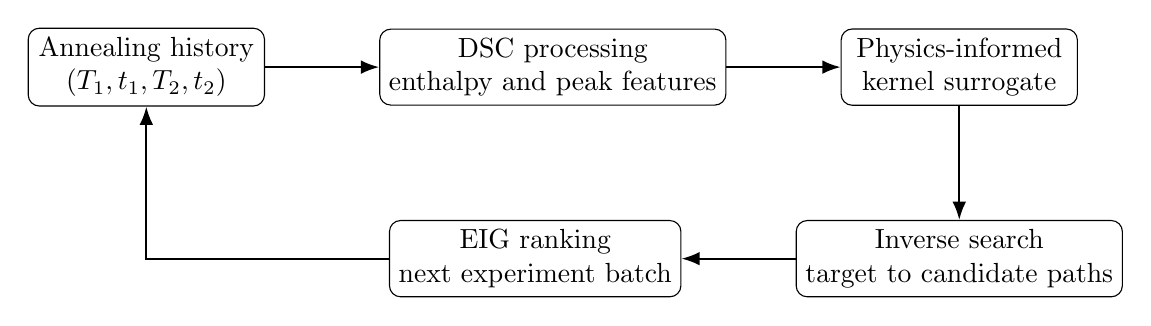
\begin{tikzpicture}[
  node distance=1.45cm,
  box/.style={draw, rounded corners, align=center, minimum width=3.0cm, minimum height=0.95cm},
  arrow/.style={-Latex, thick}
]
\node[box] (history) {Annealing history\\$(\Tone,\ToneTime,\Ttwo,\TtwoTime)$};
\node[box, right=of history] (dsc) {DSC processing\\enthalpy and peak features};
\node[box, right=of dsc] (model) {Physics-informed\\kernel surrogate};
\node[box, below=of model] (inverse) {Inverse search\\target to candidate paths};
\node[box, left=of inverse] (eig) {EIG ranking\\next experiment batch};
\draw[arrow] (history) -- (dsc);
\draw[arrow] (dsc) -- (model);
\draw[arrow] (model) -- (inverse);
\draw[arrow] (inverse) -- (eig);
\draw[arrow] (eig) -| (history);
\end{tikzpicture}
\caption{Workflow for active-learning annealing reconstruction. The present paper uses a forward surrogate as the central object and treats inverse reconstruction and experiment selection as search problems over feasible annealing histories.}
\label{fig:workflow}
\end{figure}

\section{Results}
\subsection{Current PS data set}
The present data set contains 102 usable DSC-derived samples after adding the latest PS Kovacs 03/04 batches. The usable rows comprise 45 single-step and 57 two-step annealing histories. Figure~\ref{fig:dataset} summarizes the source-file composition and the processing logic used to convert raw DSC scans into finite-time recovery descriptors.

\begin{figure}[t]
\centering
\begin{subfigure}{0.55\linewidth}
  \centering
  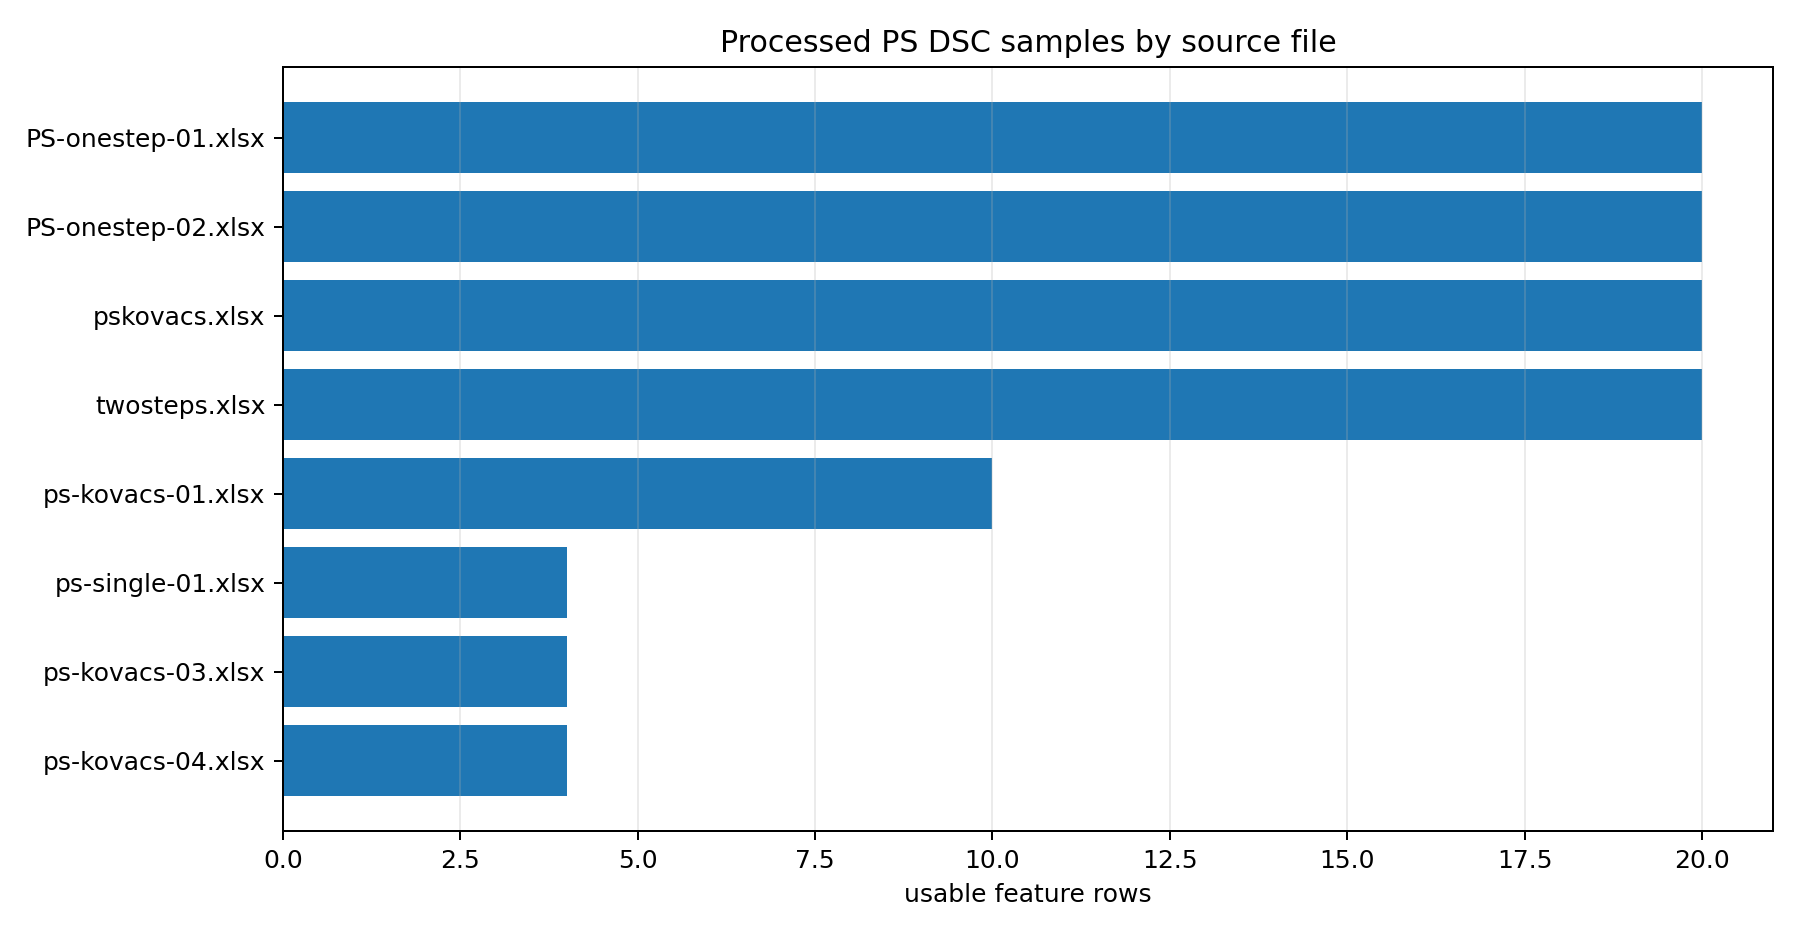
\includegraphics[width=\linewidth]{dataset_sources.png}
  \caption{Usable samples by DSC source file.}
\end{subfigure}
\begin{subfigure}{0.40\linewidth}
  \centering
  \fbox{\parbox{0.88\linewidth}{
  \textbf{Feature extraction}\\[0.35em]
  Empty/ref correction\\
  Linear detrending\\
  Peak integration\\
  $I_{\mu\mathrm{W}\,{}^{\circ}\mathrm{C}}\rightarrow\si{J/g}$\\
  Recovery and path indices
  }}
  \caption{Processing summary.}
\end{subfigure}
\caption{Experimental data and DSC processing used in the current manuscript draft. The sample mass used for enthalpy conversion is \SI{4.7}{mg}.}
\label{fig:dataset}
\end{figure}

\subsection{Forward prediction from annealing history}
The raw kernel model provides a finite-time forward predictor for the main calorimetric quantities. On the current grouped split, the test-set MAEs are \SI{0.181}{J/g} for total enthalpy recovery, \SI{0.146}{J/g} for peak area, 0.157 for recovery index, and 0.194 for path-dependence index (Table~\ref{tab:raw_metrics}). These errors are suitable for ranking experiments and comparing broad regions of the design space, but they do not imply that the inverse annealing path is uniquely determined.

\begin{table}[t]
\centering
\caption{Current raw-kernel grouped test performance.}
\label{tab:raw_metrics}
\begin{tabular}{lccc}
\toprule
Target & MAE & RMSE & $R^2$ \\
\midrule
Total enthalpy recovery (\si{J/g}) & 0.181 & 0.209 & 0.240 \\
Peak area (\si{J/g}) & 0.146 & 0.166 & 0.209 \\
Peak temperature (\si{\celsius}) & 0.346 & 0.393 & 0.276 \\
Recovery index & 0.157 & 0.173 & 0.180 \\
Path-dependence index & 0.194 & 0.233 & -0.018 \\
\bottomrule
\end{tabular}
\end{table}

\begin{figure}[t]
\centering
\begin{subfigure}{0.48\linewidth}
  \centering
  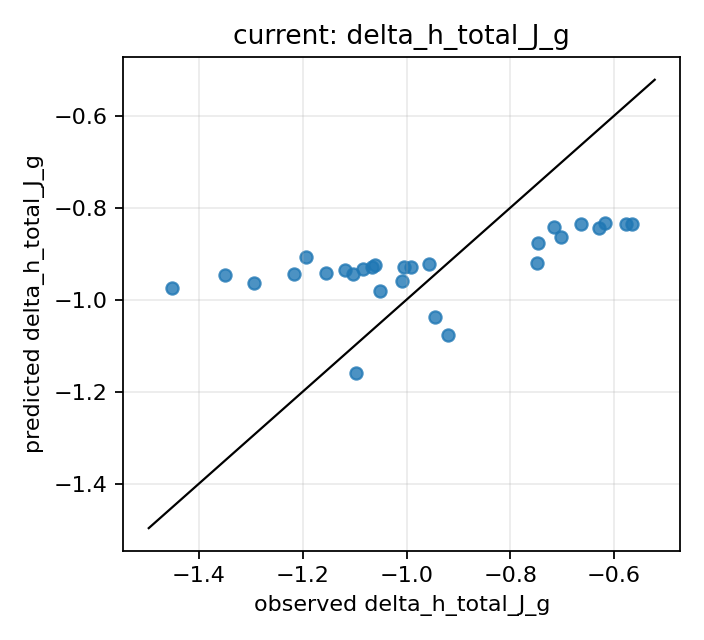
\includegraphics[width=\linewidth]{forward_delta_h_scatter.png}
  \caption{Total enthalpy recovery.}
\end{subfigure}
\begin{subfigure}{0.48\linewidth}
  \centering
  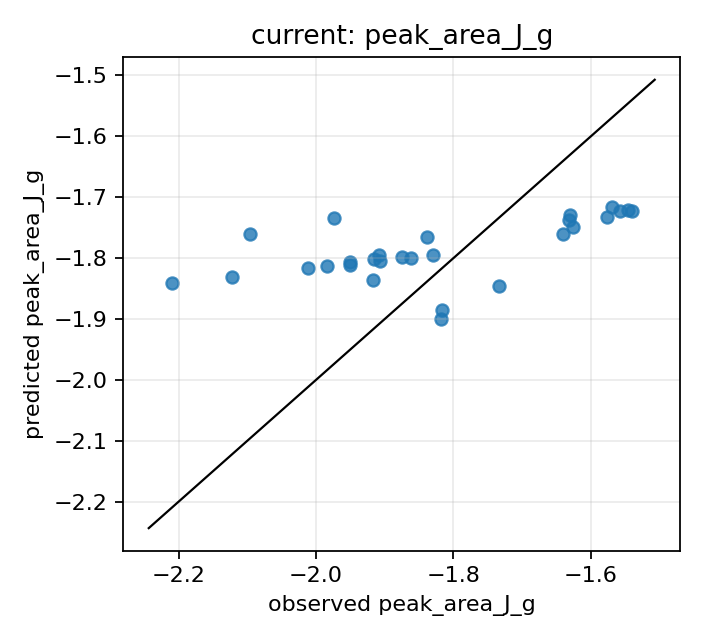
\includegraphics[width=\linewidth]{forward_peak_area_scatter.png}
  \caption{Peak area.}
\end{subfigure}
\begin{subfigure}{0.48\linewidth}
  \centering
  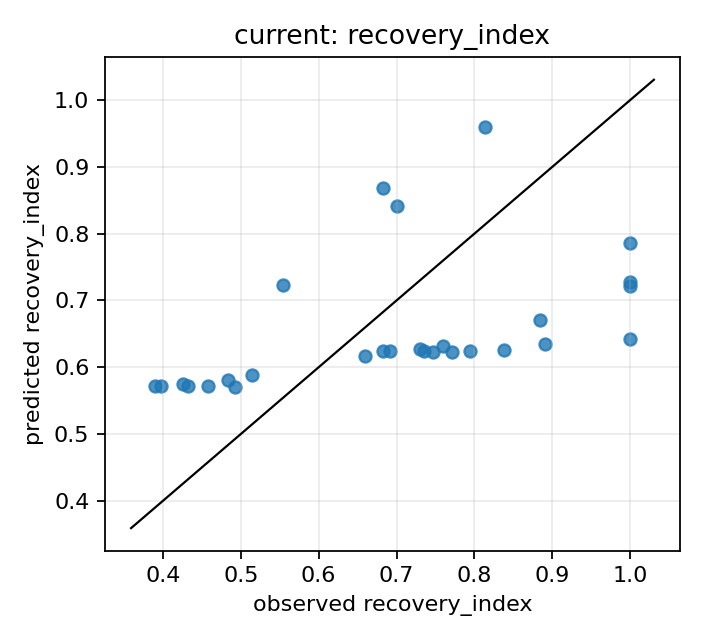
\includegraphics[width=\linewidth]{forward_recovery_index_scatter.png}
  \caption{Recovery index.}
\end{subfigure}
\begin{subfigure}{0.48\linewidth}
  \centering
  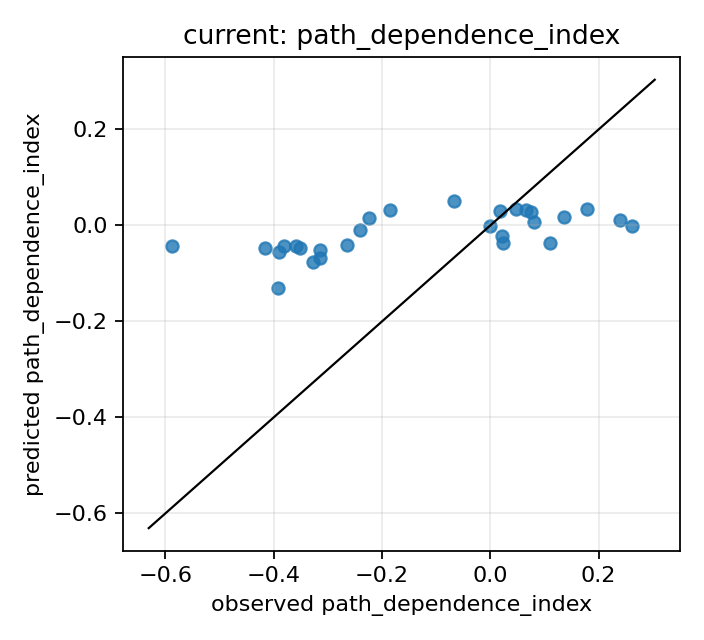
\includegraphics[width=\linewidth]{forward_path_dependence_scatter.png}
  \caption{Path-dependence index.}
\end{subfigure}
\caption{Representative forward-prediction scatter plots for current-target descriptors. These panels are used as draft placeholders for the final model-performance figure and should be regenerated from the final selected model before submission.}
\label{fig:forward}
\end{figure}

\subsection{Physics-informed surrogate improvement}
Embedding TNM-style path and dose features improves the core-target error of the kernel model on this grouped split. The selected physics-informed kernel reduces the mean MAE normalized by test-set target standard deviation from 0.7997 to 0.7352, an 8.1\% relative reduction. It improves all four core targets in the current split: total enthalpy recovery, peak area, recovery index, and path-dependence index. This result should be interpreted as a current split-level screening result rather than a final statistical ranking of all possible model classes.

\begin{figure}[t]
\centering
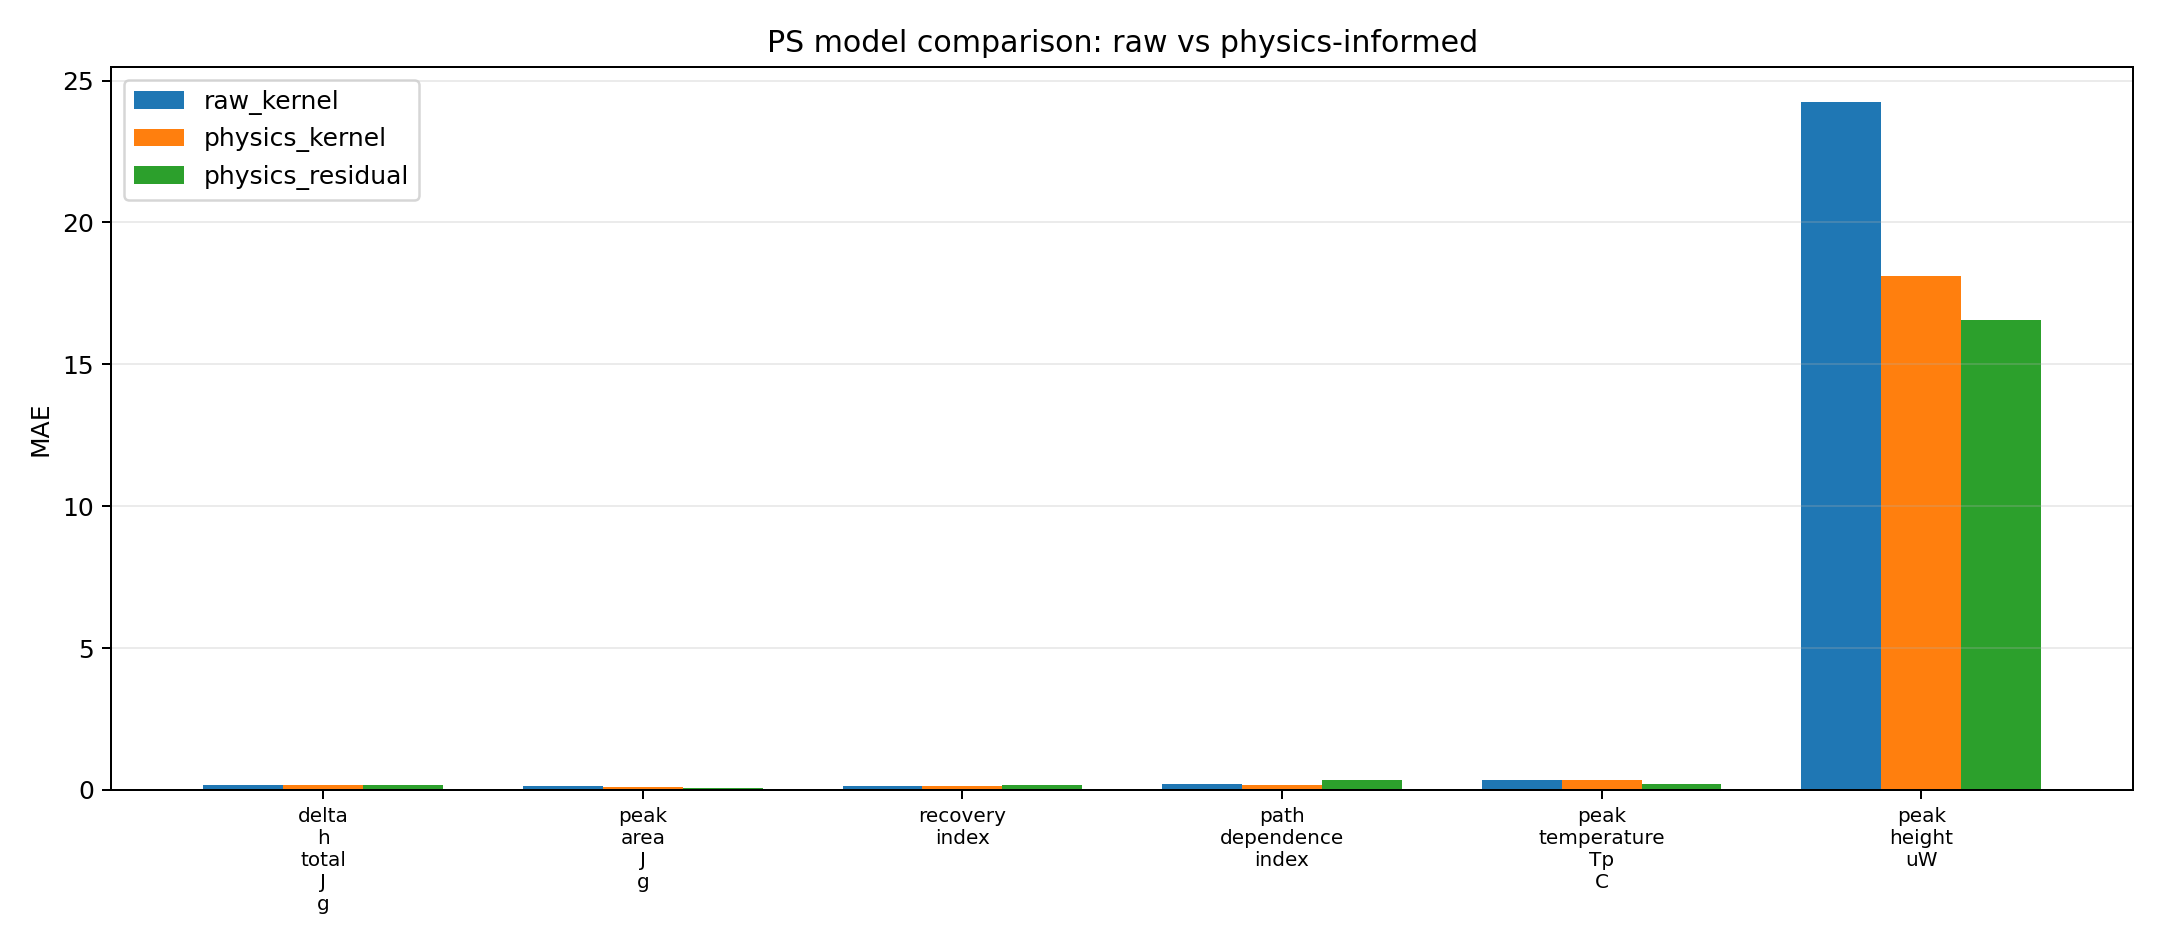
\includegraphics[width=0.78\linewidth]{physics_informed_mae_comparison.png}
\caption{Raw, physics-informed, and residual-model comparison on the same grouped split. The compact physics-informed kernel is preferred for the current active-learning loop because it improves the core targets without damaging recovery-index or path-dependence behavior.}
\label{fig:physics}
\end{figure}

\subsection{Inverse reconstruction remains underdetermined}
The inverse problem is substantially harder than the forward problem. Among 49 two-step samples, the best current inverse reconstruction rates remain low under the near-match definition. For example, in the most populated \SIrange{80}{90}{\celsius} first-step bin, the top-1 near-match rate is 0.025 and the top-10 near-match rate is 0.100. The \SIrange{50}{60}{\celsius} bin has a lower \Tone\ MAE but insufficient coverage and large time-factor errors. These results show that the model can be useful for proposing candidate histories, but not for claiming a unique four-parameter reconstruction.

\begin{figure}[t]
\centering
\begin{subfigure}{0.48\linewidth}
  \centering
  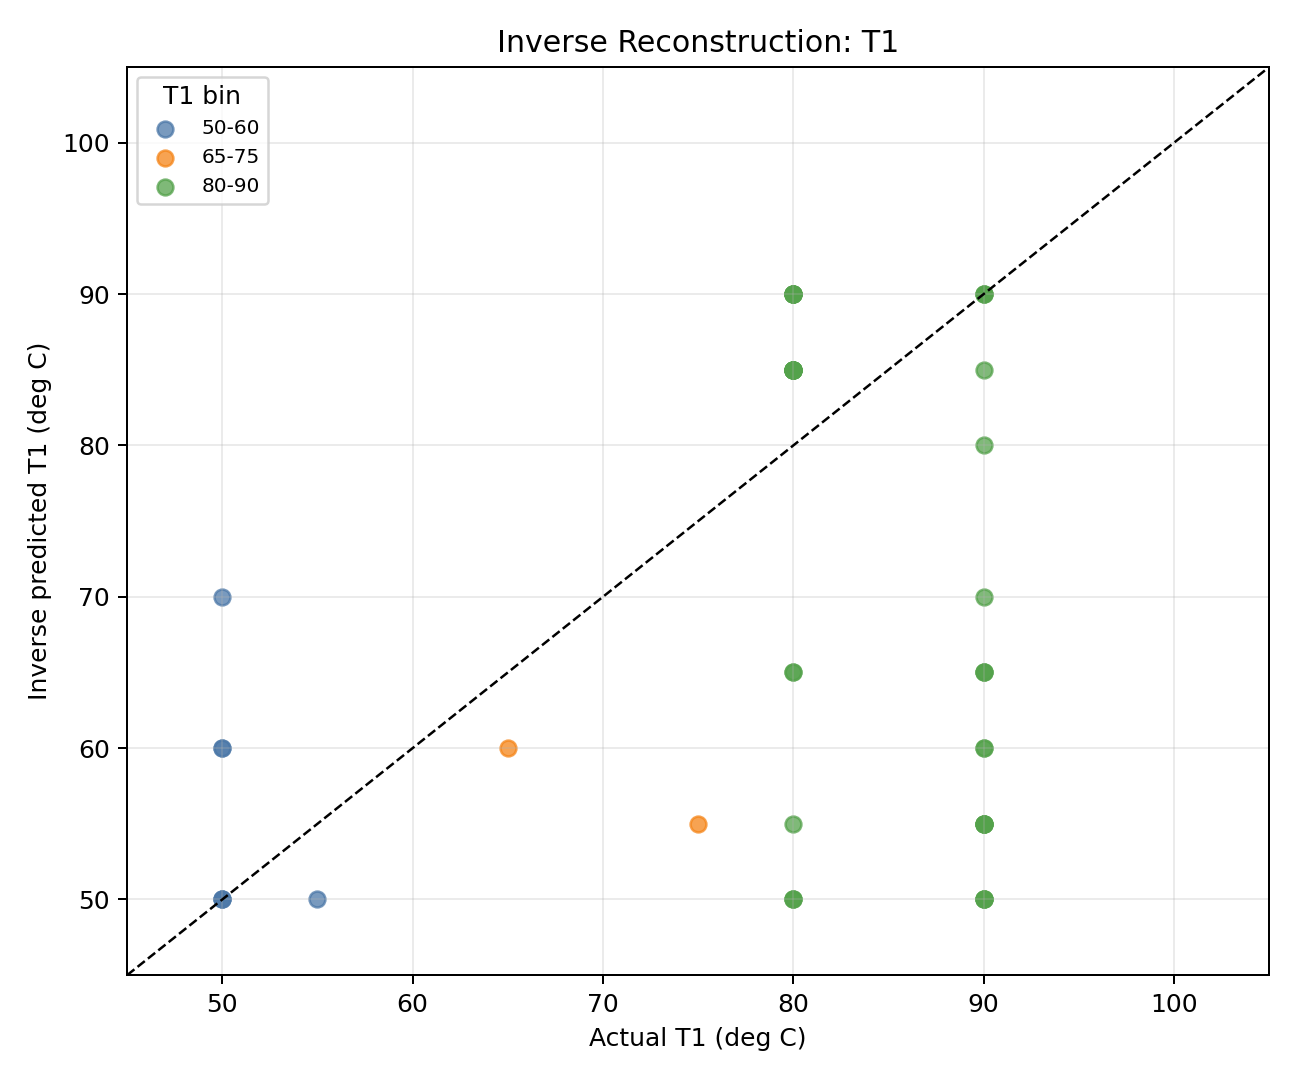
\includegraphics[width=\linewidth]{inverse_T1_actual_vs_pred.png}
  \caption{\Tone\ actual versus inverse-predicted.}
\end{subfigure}
\begin{subfigure}{0.48\linewidth}
  \centering
  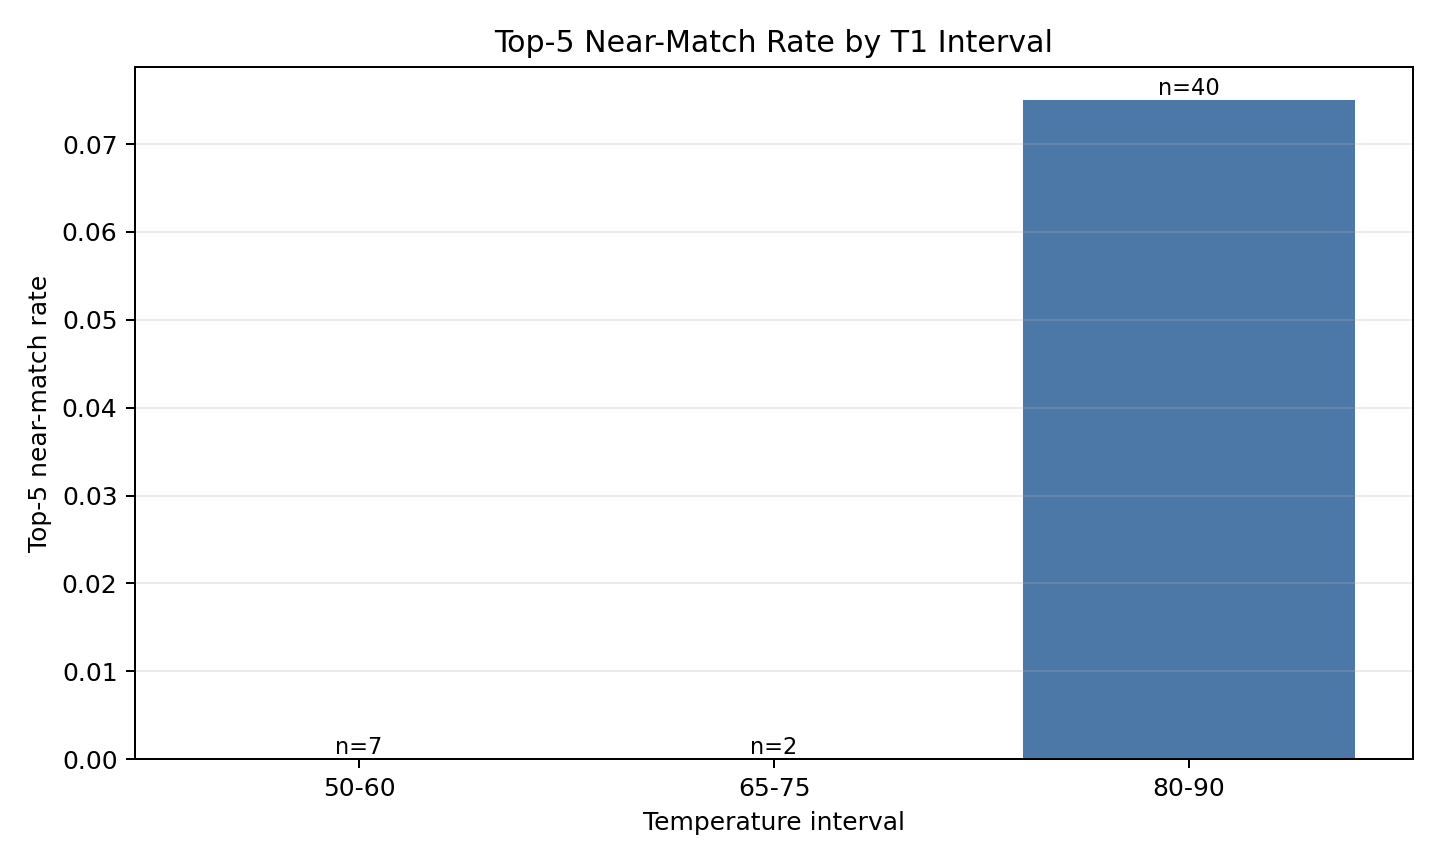
\includegraphics[width=\linewidth]{inverse_top5_rate_by_T1_bin.png}
  \caption{Top-5 near-match rate by \Tone\ bin.}
\end{subfigure}
\caption{Inverse reconstruction diagnostics. Even when forward prediction is usable, multiple annealing histories can yield similar DSC feature vectors, especially when temperature and time effects are not locally separable.}
\label{fig:inverse}
\end{figure}

\subsection{EIG-selected next experiments}
The active-learning layer ranks feasible two-step experiments by weighted information gain, novelty, time penalty, and batch redundancy. The current greedy selected two-step batch contains 18 candidates from 5346 two-step candidates. The selected conditions emphasize uncertain and novel finite-time paths, including same-temperature high-temperature probes and low-to-high temperature jumps. The score in Table~\ref{tab:eig} is therefore the greedy batch-selection score, not a pure single-candidate EIG value.

\begin{table}[t]
\centering
\caption{Top entries in the greedy EIG-selected two-step batch from the current physics-informed surrogate.}
\label{tab:eig}
\begin{tabular}{rrrrrr}
\toprule
Rank & \Tone\ (\si{\celsius}) & \ToneTime\ (s) & \Ttwo\ (\si{\celsius}) & \TtwoTime\ (s) & Score \\
\midrule
1 & 100 & 100 & 100 & 100 & 1.692 \\
2 & 70 & 900 & 100 & 300 & 1.677 \\
3 & 50 & 100 & 100 & 10 & 1.650 \\
4 & 50 & 30 & 100 & 100 & 1.654 \\
5 & 70 & 1800 & 70 & 300 & 1.633 \\
6 & 100 & 10 & 100 & 30 & 1.660 \\
7 & 100 & 1800 & 100 & 10 & 1.638 \\
8 & 70 & 60 & 100 & 60 & 1.626 \\
\bottomrule
\end{tabular}
\end{table}

\begin{figure}[t]
\centering
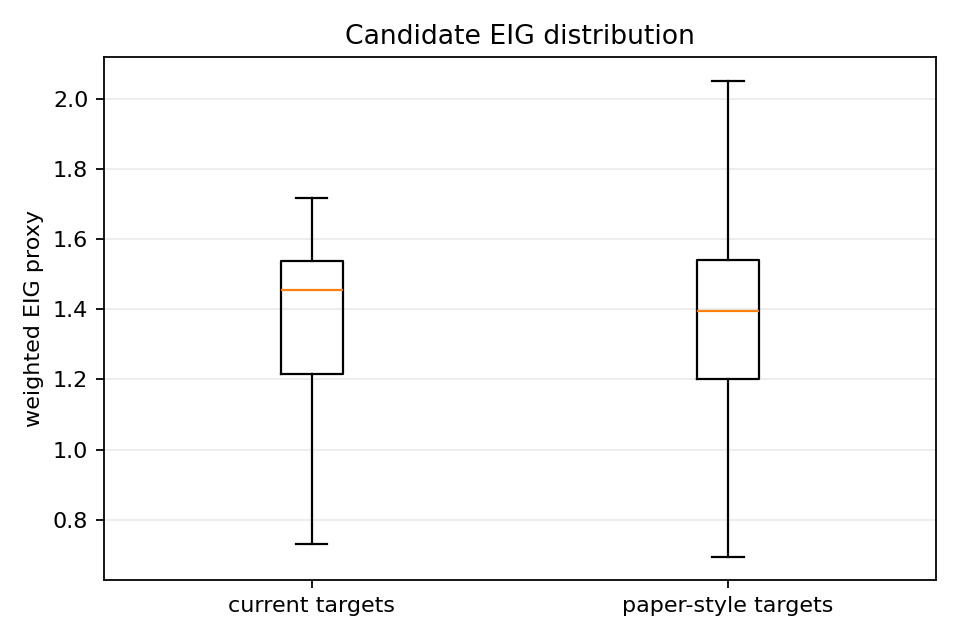
\includegraphics[width=0.70\linewidth]{eig_distribution_targets.png}
\caption{Draft comparison of EIG distributions under current PS targets and paper-style kinetic targets. The paper-style target set is useful as a diagnostic but currently depends on effective \Sstar/\Hstar\ proxy labels rather than direct multi-rate measurements.}
\label{fig:eig_distribution}
\end{figure}

\subsection{Paper-style kinetic targets}
A reduced paper-style target set, consisting of $\Delta h$, peak enthalpy, effective \Sstar, and effective \Hstar, lowers the normalized error summary relative to the full current target set in the same split. However, the current effective \Sstar/\Hstar\ labels are inferred from annealing time and peak position rather than directly measured from repeated heating-rate experiments. A strict ARRT/Kissinger analysis inspected 103 recovery scans and 82 annealed-state groups but found zero groups with the required three distinct heating rates. Thus, direct \Sstar/\Hstar\ training remains a planned experimental extension, not a completed result.

\subsection{Planned post-EIG validation}
\fbox{\parbox{0.92\linewidth}{
\textbf{Planned validation figure placeholder.}
After the next EIG-selected batch is measured, this section will compare pre- and post-batch errors for the physics-informed model, regenerate the forward-prediction scatter plots, quantify whether path-dependence uncertainty decreases, and test whether any selected repeated heating-rate conditions unlock direct \Sstar/\Hstar\ estimates. No post-EIG experimental result is claimed in this draft.
}}

\section{Discussion}
The current results support three working conclusions, all subject to the small data set and grouped-split dependence of the present analysis. First, finite-time PS enthalpy recovery can be screened for experiment ranking using a sparse kernel surrogate, especially when the feature space includes physically motivated dose and path descriptors. Second, inverse reconstruction is not solved by forward accuracy alone. The low top-$k$ near-match rates reflect a practical identifiability problem: multiple time-temperature histories can occupy similar regions of DSC feature space. Third, the correct role of active learning is not merely to maximize recovery amplitude, but to choose experiments that separate confounded temperature, time, and path effects.

This framing also clarifies how the present approach relates to activation-entropy descriptions of glass memory. The Song et al. framework suggests that \Sstar\ and \Hstar\ can be powerful kinetic coordinates for memory effects \citep{song2020activation}. In the current PS data, however, direct use of these coordinates is limited by the lack of repeated heating-rate measurements for identical annealed states. The responsible interpretation is therefore to treat current \Sstar/\Hstar\ quantities as effective diagnostic proxies, while using TNM-style dose features as a lower-risk way to inject physical prior information into the surrogate model.

The next EIG-selected experiments should be judged by whether they improve identifiability, not only by whether they reduce aggregate MAE. Especially valuable additions will form local grids around high-uncertainty paths, include controlled repeats for noise estimation, and add selected multi-heating-rate triplets for direct kinetic-coordinate extraction.

\section{Conclusion}
This draft establishes a physics-informed active-learning manuscript framework for PS finite-time enthalpy-recovery reconstruction. The present data support a forward surrogate and show a measurable benefit from TNM-inspired features, while inverse four-parameter reconstruction remains underdetermined. The proposed EIG loop turns that limitation into an experiment-design objective: select the next annealing histories that most efficiently reduce uncertainty and separate path effects. The paper should therefore be presented as a closed-loop experimental methodology, with the post-EIG validation batch intended to complete the final evidence chain.

\section*{Data and code availability}
The analysis scripts, processed feature tables, model payloads, and figure assets are maintained in the accompanying project repository. This section should be replaced with a permanent repository URL before submission.

\section*{Acknowledgements}
Acknowledgements will be added after the author list, funding sources, and instrument access details are finalized.

\bibliographystyle{unsrtnat}
\bibliography{references}

\end{document}
